\documentclass{article}

\usepackage{times}
\usepackage{epsfig}
\usepackage{graphicx}
\usepackage{amsmath}
\usepackage{amssymb}
\usepackage{listings}
\usepackage{float}
\usepackage{subfigure}

\usepackage[preprint]{neurips_2021}

\usepackage[utf8]{inputenc} % allow utf-8 input
\usepackage[T1]{fontenc}    % use 8-bit T1 fonts
\usepackage{hyperref}       % hyperlinks
\usepackage{url}            % simple URL typesetting
\usepackage{booktabs}       % professional-quality tables
\usepackage{amsfonts}       % blackboard math symbols
\usepackage{nicefrac}       % compact symbols for 1/2, etc.
\usepackage{microtype}      % microtypography
\usepackage{xcolor}         % colors

\title{Project of CS182 \\ 
    Image Super Resolution \\
    Application On Remote Sensing Dataset}

\author{
    Bi Chunhao \\
    \texttt{bichh@shanghaitech.edu.cn} \\
    \And
    Jiang Yichen \\
    \texttt{jiangych1@shanghaitech.edu.cn} \\
}

\begin{document}

\maketitle

\begin{abstract}
    This is the final project of CS182, here we focused on a specific application called Image Super Resolution,
    which generates a higher resolution images based on the raw input. 
    We compared several existing algorithms and carried out some experiments to find the most suitable solution.
\end{abstract}

\section{Introduction}
Super-resolution(SR) technology is a technology to restore a high-resolution(HR) picture from a low-resolution(LR). 
With the appearance of neural network, some new SR method based on deep neural network achieve better performance than traditional algorithm. 
Thus SR is followed with interest in many field, one typical field is remote sensing. 
Quality of remote sensing images is inevitably affected by accuracy of current sensors and complex atmospheric conditions. 
Neural network based super-resolution technology, although not so mature for now, have potential to help solve these problems. 
In our project, we will test and compare some cutting-edge network algorithms on super-resolution of remote sensing image. 
  
\section{Related Work}
  Since the appearance of SRCNN $[6]$, many achievements on combination of SR and neural network has been made by researchers. 
  As FSRCNN $[1]$ and ESPCN $[2]$, which is based on CNNs, has simple structure and reasonable computation complexity. 
  LapSRN $[3]$ has multiple level CNNs structure. 
  EDSR $[4]$ are motivated by ResNet $[7]$, which is proposed dealing with vanishing gradient problem caused when more layers are added to the network.
  Recent research direction is to extend depth of the network and the amount of training sets to achieve better SR performance.
  However, with the model being deeper and deeper, the time cost also increases.
  
  \section{Different solutions} 
  \subsection{Bicubic}
  Bicubic is an classical interpolation method. In this project, Bicubic method is used to compare with other methods.
  It may be the slowest in the three mentioned, but still is much faster compared to the methods using CNN.
  
  \subsection{FSRCNN} 
  FSRCNN$[1]$ is accelerated version of SRCNN$[6]$, 
  which directly take LR image as the input and conducts upsampling by the deconvolution layer at the end of the net work instead of upscales LR image before entering the network. 
  This change leads to 2 main difference: 1. Directly, no need to cost time carrying out Bicubic operation. 
  2. Conv operation on LR image is less costly, With less computational complexity, 
  FSRCNN can support a deeper network and achieve a better effect.
  
  FSRCNN take PReLU as the activation function and L2 as loss.


  \subsection{ESPCN}
  ESPCN$[2]$ is also motivated by SRCNN$[6]$, like FSRCNN$[1]$, 
  ESPCN takes LR image as the input and have low computational complexity. 
  And ESPCN have a efficient sub-pixel convolution layer for learn.
  
  ESPCN take $tanh()$ as activation function and L2 as loss.

  \begin{figure}[H]
    \begin{minipage}[H]{0.5\linewidth}
    \centering
    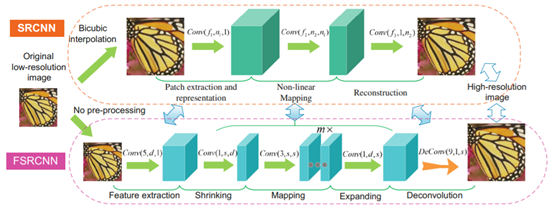
\includegraphics[width=2.7in]{images/FSRCNN.png}
    \caption{The network structure of SRCNN and FSRCNN}

    \end{minipage}
    \begin{minipage}[H]{0.5\linewidth}
    \centering
    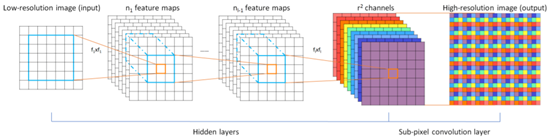
\includegraphics[width=2.7in]{images/ESPCN.png}
    \caption{The network structure of ESPCN}

    \end{minipage}
\end{figure}

  \subsection{LapSRN}
  LapSRN$[3]$ has multiple-level structure. Every level onduct a 2x upscaling on input 
  image and output of previous level can be taken as input of next level. As a result LapSRN can support up to 8x upscaling. 
  
  LapSRN take L1 as loss, which is optimized at end of every level.
  
  \subsection{EDSR}
  The design of EDSR$[4]$ is based on the SRResNet$[8]$. 
  The author team remove the BN layers and achieve better performance and memory usage. 
  EDSR has won NTIRE2017 SR Challenge.

  EDSR use L1 loss instead of L2, because author team find L1 loss provides better conver-gence.
  
  \begin{figure}[H]
    \begin{minipage}[H]{0.5\linewidth}
    \centering
    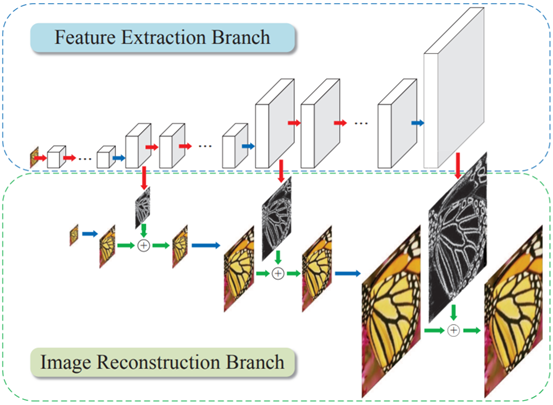
\includegraphics[width=2.7in]{images/LapSRN.png}
    \caption{The network structure of LapSRN}

    \end{minipage}
    \begin{minipage}[H]{0.5\linewidth}
    \centering
    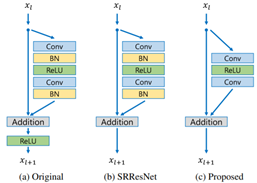
\includegraphics[width=2.7in]{images/EDSR1.png}
    \caption{Comparison of residual blocks in ResNet, SRResNet and EDSR}

    \end{minipage}
\end{figure}

  \section{Results and Experiments}
  \subsection{Testing}
  \subsubsection*{Models}
  Due to time and equipments limitations, we can't train all the models by ourselves, so
  we take the $\times 4$ version trained models of 
  \href{https://github.com/Saafke/EDSR_Tensorflow/tree/master/models}{EDSR},
  \href{https://github.com/Saafke/FSRCNN_Tensorflow/tree/master/models}{FSRCNN},
  \href{https://github.com/fannymonori/TF-ESPCN/tree/master/export}{ESPCN},
  \href{https://github.com/fannymonori/TF-LapSRN/tree/master/export}{LapSRN} from GitLab.
  Real-ESRGAN's model doesn't join the following experiment. 
  Team of Real-ESRGAN provide their own executable file with hardware acceleration, convenient but can't match our requirement.
  
  \subsubsection*{Evaluation Metrics}

    \subsubsection{PSNR}    
      PSNR (Peak Signal to Noise Ratio) is a generally used measuring method for image resolution.
      PSNR is the ratio of maximum signal power and the average power.
      The definition is:
      \begin{align*}
          PSNR = 10log_{10}\frac{MaxValue^2}{MSE} = 10log_{10}\frac{255}{MSE}
      \end{align*}
      Where MSE(Mean Squared Error) denotes the average power between the groundtruth and the result image.
  
      However, PSNR scores is not consistent to the quality human eye perceives, sometimes a higher PSNR score image may look worse.
      The reason is that human eye is not sensitive to high frequency noise, which is usually separately distributed. 
      The perception is influenced by the whole surrounding area in a low frequency way.
  
    \subsubsection{SSIM}   
      SSIM (Structural Similarity Index) is a method to evaluate the similarity of two images.
      It is based on the whole structure, with less focus on pixelwise error. 
      SSIM contains three evaluation aspects: Luminance, Contrast and Structure.
      The detailed calculation is complicated. A general pipeline is as follows:
      \begin{figure}[H]
          \centering
          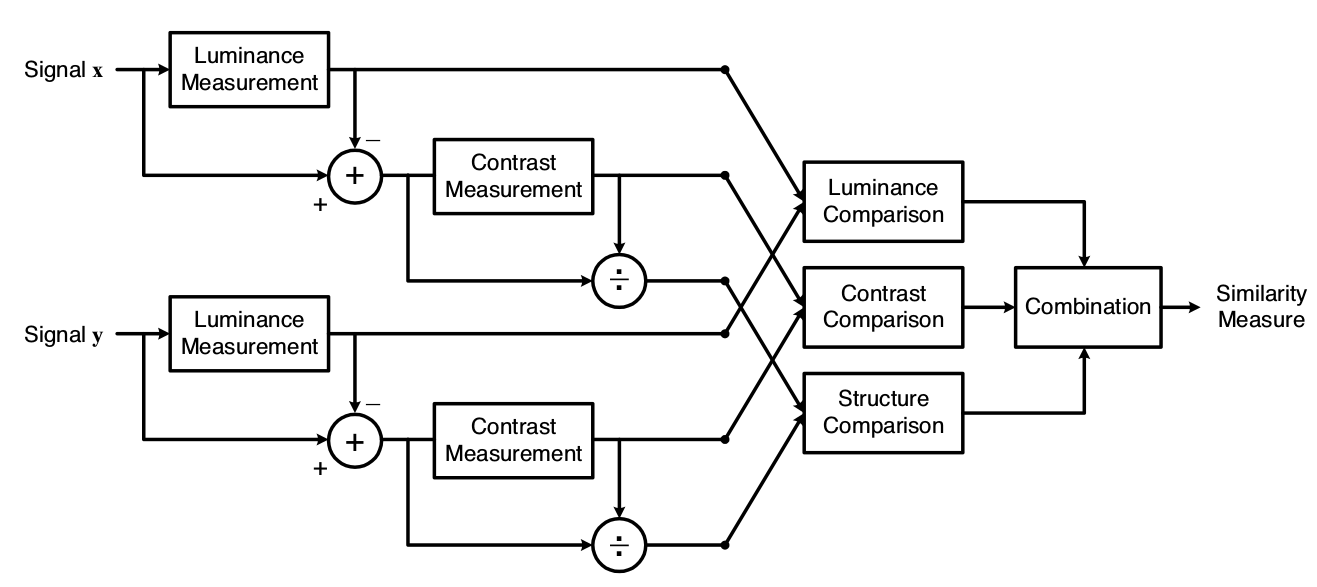
\includegraphics[scale = 0.2]{images/SSIM.png}
          \caption{Same PSNR scores with different distortions}
      \end{figure}
      The Luminance can be represented as mean value, the Contrast as variance after normalization, 
      and the structure as coefficient of association (fraction of covariance and variance products).
  

  \subsection{Results}
  The testing set we take is DIV2K High Resolution dataset \href{https://data.vision.ee.ethz.ch/cvl/DIV2K}{DIV2K\_valid\_HR} 
  which contains 100 2K images, and negative-image-set in \href{https://hyper.ai/datasets/5422}{NWPU VHR-10} which contains 1K images taken from remote sensors.
  The former is a mixture set of varieties of objects, so we considered it as a general case.
  NWPU VHR-10 data set is a challenging ten-class geospatial object detection data set, images of which are mostly come from remote sensing equipments. 
  For this, we randomly selected an area of size $256\times 256$ for each image to test.
  We first downsample the images to 1/4 size, and then use the model to generate images with origin resolution.
  The evaluation result is calculated with the groundtruth image.
  The average scores are as follows:

  \begin{table}[H]
      \centering
      \makeatletter\def\@captype{table}\makeatother\caption{Image Evaluation on DIV2K valid HR and NWPU VHR-10}
      \begin{tabular}{cccc|cccc}
      \hline
      \multicolumn{4}{c|}{DIV2K valid HR}      & \multicolumn{4}{c}{NWPU VHR-10}\\\hline
      Algorithm & PSNR   & SSIM   & Time cost  & Algorithm & PSNR   & SSIM   & Time cost  \\ \hline
      Bicubic   & 26.228 & 0.7722 & 0.0025     & Bicubic   & 28.679 & 0.7591 & 0.0003     \\ \hline
      EDSR      & 27.789 & 0.8091 & 34.844     & EDSR      & 30.090 & 0.7972 & 1.0144     \\ \hline
      ESPCN     & 26.689 & 0.7737 & 0.0840     & ESPCN     & 28.882 & 0.7589 & 0.0040     \\ \hline
      FSRCNN    & 26.580 & 0.7704 & 0.1302     & FSRCNN    & 28.647 & 0.7556 & 0.0038     \\ \hline
      LapSRN    & 26.710 & 0.7741 & 2.9266     & LapSRN    & 28.915 & 0.7589 & 0.0739     \\ \hline
      \end{tabular} 
  \end{table}

  To be noticed, EDSR results in a great accuracy. 
  However, due to the great size of its network, it also spent a lot of time than the others.
  
  \subsection{Visualization}
  If the scores are not familiar, some visual results can bring a more intuitive understanding.
\begin{figure}[H]
    \centering
    \subfigure[Groundtruth]{
    \begin{minipage}[t]{0.13\linewidth}
    \centering
    
\includegraphics[width=0.65in]{images/plant_origin.png}
    \end{minipage}
    }
    \subfigure[Bicubic]{
    \begin{minipage}[t]{0.13\linewidth}
    \centering
    
\includegraphics[width=0.65in]{images/plant_bicubic.png}
    \end{minipage}
    }
    \subfigure[EDSR]{
    \begin{minipage}[t]{0.13\linewidth}
    \centering
    
\includegraphics[width=0.65in]{images/plant_EDSR.png}
    \end{minipage}
    }
    \subfigure[ESPCN]{
    \begin{minipage}[t]{0.13\linewidth}
    \centering
    
\includegraphics[width=0.65in]{images/plant_ESPCN.png}
    \end{minipage}
    }
    \subfigure[FSRCNN]{
    \begin{minipage}[t]{0.13\linewidth}
    \centering
    
\includegraphics[width=0.65in]{images/plant_FSRCNN.png}
    \end{minipage}
    }
    \subfigure[LapSRN]{
    \begin{minipage}[t]{0.13\linewidth}
    \centering
    
\includegraphics[width=0.65in]{images/plant_LapSRN.png}
    \end{minipage}
    }
    \caption{Remote sensing pictures restoration}
\end{figure}

  From the result above, we can tell that the model is useful for dealing with aliasing.
  Aliasing is a normal consequence when pictures are compressed into a lower resolution.
  The bicubic interpolation can't do well with this situation, 
  but the rest four CNN methods can smoothen the images to be more realistic.
  If the images compressed after Gaussian kernel convolution,
  then the aliasing effect will be reduced, and thus there is no much difference between bicubic method and the others.
  In this case, bicubic method is better for its low time cost and quite good result.
  
  As for remote sensing image restoration.
  We tested the models on such dataset. 
  Some visual results are shown here:

  The LR image is generated from an HR one using nearest Neighbor method in opencv.
  Then the image is considered as the input in the testing algorithms.
  The result after the models are:
  \begin{figure}[H]
      \centering
      \subfigure[Groundtruth]{
      \begin{minipage}[t]{0.13\linewidth}
      \centering
      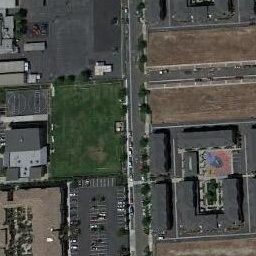
\includegraphics[width=0.65in]{images/rs_origin.png}
      \end{minipage}
      }
      \subfigure[Bicubic]{
      \begin{minipage}[t]{0.13\linewidth}
      \centering
      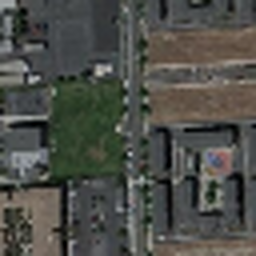
\includegraphics[width=0.65in]{images/rs_bicubic.png}
      \end{minipage}
      }
      \subfigure[EDSR]{
      \begin{minipage}[t]{0.13\linewidth}
      \centering
      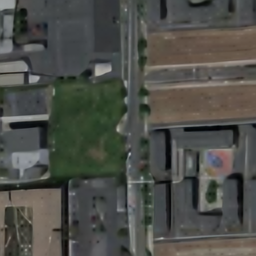
\includegraphics[width=0.65in]{images/rs_EDSR.png}
      \end{minipage}
      }
      \subfigure[ESPCN]{
      \begin{minipage}[t]{0.13\linewidth}
      \centering
      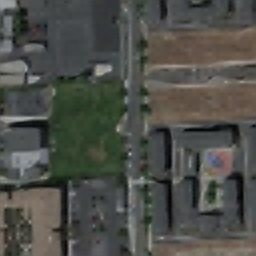
\includegraphics[width=0.65in]{images/rs_ESPCN.png}
      \end{minipage}
      }
      \subfigure[FSRCNN]{
      \begin{minipage}[t]{0.13\linewidth}
      \centering
      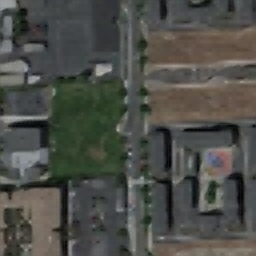
\includegraphics[width=0.65in]{images/rs_FSRCNN.png}
      \end{minipage}
      }
      \subfigure[LapSRN]{
      \begin{minipage}[t]{0.13\linewidth}
      \centering
      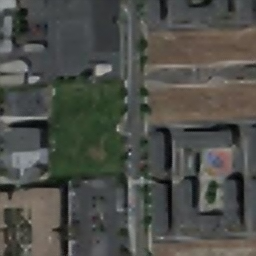
\includegraphics[width=0.65in]{images/rs_LapSRN.png}
      \end{minipage}
      }
      \caption{Restoration from aliased compression}
  \end{figure}

  \subsubsection*{Conclusion}
  CNN methods can deal with aliasing effect, which is mentioned above.
  From the visual results, we can also tell that there are information differences between the ground truth image and the restored ones.
  Although different algorithms carried out difference results, CNN methods generally tend to smoothen the image.
  The smoothened images have more clear edge representations and the building blocks are generally more clear, with fewer details and more regular shapes.
  Some high frequency details are omitted, which are not important here, and the low frequency components are kept in the results.
  The filtering ability makes CNN a better solution in some cases of usage.

\section*{References}

[1] C. Dong, C. C. Loy, and X. Tang. Accelerating the super-resolution convolutional neural network. In ECCV, 2016. 

[2] W. Shi, J. Caballero, F. Huszar, J. Totz, A. Aitken, R. Bishop, D. Rueckert, and Z. Wang. Real-time single image and video super-resolution using an efficient sub-pixel convolutional neural network. In CVPR, 2016.

[3] W.-S. Lai, J.-B. Huang, N. Ahuja, and M.-H. Yang. Deep laplacian pyramid networks for fast and accurate superresolution. In CVPR, 2017.

[4] B. Lim, S. Son, H. Kim, S. Nah, and K. M. Lee. Enhanced deep residual networks for single image super-resolution. In CVPRW, 2017.

[5] Xintao Wang, Liangbin Xie, Chao Dong, and Ying Shan. Real-esrgan: Training real-world blind super-resolution with pure synthetic data. arXiv preprint arXiv:2107.10833, 2021.

[6] Dong, C., Loy, C.C., He, K., Tang, X.: Learning a deep convolutional network for image super-resolution. In: Fleet, D., Pajdla, T., Schiele, B., Tuytelaars, T. (eds.) ECCV 2014, Part IV. LNCS, vol. 8692, pp. 184–199. Springer, Heidelberg (2014)

[7] K. He, X. Zhang, S. Ren, and J. Sun. Deep residual learning for image recognition. In CVPR, 2016.

[8] Ledig, C., Theis, L., Husz´ar, F., Caballero, J., Cunningham, A., Acosta, A., Aitken, A., Tejani, A., Totz, J., Wang, Z., et al.: Photo-realistic single image superresolution using a generative adversarial network. In: CVPR (2017)

[9] D. Yang, Z. Li, Y. Xia and Z. Chen, “Remote sensing image super-resolution: Challenges and approaches,” 2015 IEEE International Conference on Digital Signal Processing (DSP), 2015, pp. 196-200, doi: 10.1109/ICDSP.2015.7251858.

[10] T. Wang, W. Sun, H. Qi and P. Ren, “Aerial Image Super Resolution via Wavelet Multiscale Convolutional Neural Networks,” in IEEE Geoscience and Remote Sensing Letters, vol. 15, no. 5, pp. 769-773, May 2018, doi: 10.1109/LGRS.2018.2810893.




\end{document}